%
% Szakdolgozatminta az Eszterházy Károly Katolikus Egyetem
% matematika illetve informatika szakos hallgatóinak.
%

\documentclass[
% opciók nélkül: egyoldalas nyomtatás, elektronikus verzió
% twoside,     % kétoldalas nyomtatás
% tocnopagenum,% oldalszámozás a tartalomjegyzék után kezdődik
]{thesis-ekf}
\usepackage[T1]{fontenc}
\PassOptionsToPackage{defaults=hu-min}{magyar.ldf}
\usepackage[magyar]{babel}
\usepackage{mathtools,amssymb,amsthm,pdfpages}
\footnotestyle{rule=fourth}
\usepackage{float}
\usepackage{graphicx}
\usepackage{braket}

\newtheorem{tetel}{Tétel}[chapter]
\theoremstyle{definition}
\newtheorem{definicio}[tetel]{Definíció}
\theoremstyle{remark}
\newtheorem{megjegyzes}[tetel]{Megjegyzés}

\begin{document}
\institute{Matematikai és Informatikai Intézet}
\title{Tanulás segítő program és applikáció egy kvantumbites logikai kapukhoz}
\author{Bakos Rózsa Ajándék\\Programtervező informatikus BSc}
\supervisor{Dr. Biró Csaba\\Egyetemi docens}
\city{Eger}
\date{2024}
\maketitle
\tableofcontents

\chapter*{Bevezetés}
\addcontentsline{toc}{chapter}{Bevezetés}
A kvantuminformatika térhódítása egyre nagyobb figyelemnek örvend, valamint új lehetőségei hatalmas potenciállal bírnak a számítástechnika terén. A kvantummechanika alapelveinek felhasználása új típusú megoldásokat eredményez, amelyek képesek áthidalni a jelenleg is használt számítógépek korlátait. Ennek köszönhetően ezek a kvanumszámítógépek olyan problémák megoldásában ígérkeznek hatékonyabbnak, amelyek a hagyományos számítógépek számára nehezen, vagy egyáltalán nem megoldhatók.

A kvantumszámítógépek potenciális alkalmazási területei közé tartozik a mesterséges intelligencia, kriptográfia, gyógyszerkutatás és a számításelmélet. Azonban az ilyen rendszerek működése rendkívül érzékeny a környezeti tényezőkre, például gyakran használnak extrém alacsony hőmérsékletet követelő szupravezetőket. A jelenleg létező kvantumszámítógépek egyelőre kezdeti fázisban járnak, de a különböző cégek, kutatócsoportok között kialakult verseny ezen a helyzeten bármikor változtathat.

A kvantum-számítástechnika egyik kulcsfontosságú területe a kvantum logikai kapuk koncepciója, amelyek a kvantum bitek (más néven qubit) manipulációját teszik lehetővé. Ehhez a már említett kvantummechanika alapelveire támaszkodnak. Értelmezésük, valamint a hozzá tartozó összetett matematikai háttér sok esetben nehézséget okozhat.

Szakdolgozatom célja, hogy bemutasson ezen problémák áthidalására egy olyan tanulás segítő programot, mely közelebb hozza az érdeklődőkhöz a kvantumkapuk koncepcióját. Ezt egyqubites kapuk bemutatásával teszem meg. Az alkalmazás tervezése és implementálása során figyelembe veszem a felhasználók igényeit és a pedagógiai célokat, miközben kihasználom a kvantumtechnológia által nyújtott lehetőségeket.

A továbbiakban bemutatom a kvantuminformatika alapjait, a kvantumlogikai kapuk működését és jellemzőit, valamint részletesen ismertetem a fejlesztett tanulás segítő programot, beleértve annak tervezési alapelveit, implementációját és tesztelését. Végül összefoglalom az elért eredményeket és felvázolom a jövőbeli kutatási irányokat ezen a területen.

\chapter{Kvantuminformatika}
\section{Előzmények}
A kvantummechanika gyökerei az 1800-as évek elejére vezethetők vissza, ahol a fizika többek között olyan problémákkal is küzdött, mint a hőmérsékleti sugárzás.

Az első matematikai modellt, amely erre magyarázatot adott, Max Planck német fizikushoz kötjük. A ma már Planck-féle kvantumhipotézisnek ismert levezetés 1900-ban történt előterjesztésre. Ezt a dátumot tekintjük a "régi" kvantumelméleti korszak kezdetének, valamint a kvantumfizika születésének. A jelenséggel Albert Einstein is foglalkozott, aki 1905-ben megjelent, fényelektromos jelenségről szóló cikkében a már említett hőmérsékleti sugárzástól független is alkalmazta a Planck-féle kvantumhipotézist.

Ezután rohamos növekedésnek kezdett a tudományág. A "régi" kvantumelméleti korszak végét 1924-re datáljuk, amikor De Brogile publikálta anyaghullámokról szóló elméletét. A modern kvantummechanika születése 1925-ben történt, jelenleg is ebben a korszakban vagyunk.

Természetesen az informatikát sem kerülte el ez a hullám. 1981-ben Richard Feynman előadásában felvetette egy kvantumelveken működő számítógép ötletét, ami képes kvantumrendszereket szimulálni. Az ő nevéhez fűződik a kvantumszámítógép kifejezés. A korszak hasonlóan fontos neve még Paul Benioff, aki 1982-ben publikált, tanulmányában lefektette a kvantumszámítási modellek alapjait. Feynman és Benioff gondolatait felhasználva 1985-ben David Deutsch bemutatta tanulmányában egy kvantumszámítógép elméleti működését, ami képes elvégezni a klasszikus számítógép számításait, de kihasználva a kvantummechanika előnyeit. Fontos személy volt még ebben az időszakban Peter Shor, aki 1994-ben megalkotott egy olyan kvantumalgoritmust, ami a napjainkban használt titkosítási eljárásokat veszélybe sodorhatja. Az 1994-2000-es időszakban számos hasonlóan fontos kvantumalgoritmusok született. Ilyen például az 1996-ban készült Grover algoritmus, ami a rendezetlen adatokban való keresést segítette.

Ahogy ezek a felfedezések egyre tovább bővítették a kvantumszámítás fogalmát, úgy felmerült az igény a kvantumlogikai kapukra is. Az 1980-as évek végétől kezdve számos kaput állítottak elő.
\section{Jelenlegi helyzet}
A 21. században kialakult egy verseny a kutatóintézetek és tech óriások közt, cél egy kvantumszámítógép megépítése volt. Ehhez a korszakhoz fűződik a kvantumfölény kifejezés is. Ez arra utal, hogy egy kvantumszámítógép képes megoldani egy olyan problémát, melyre klasszikus társai nem képesek lehetséges időn belül.

2011-ben a D-Wave Systems cég volt az első, akik azt állították, hogy megépítették az első kereskedelmi forgalomban kapható kvantumszámítógépet, a D-Wave One-t, ami 128 qubites lapkakészleten működött.

Fontos esemény volt még a 2019-ben a Google által bejelentett kvantumfölény. 53 qubites Sycamore processzorával rendelkező kvantumszámítógépük 200 másodperc alatt megoldott egy konkrét problémát, amelyhez egy klasszikus szuperszámítógépnek körülbelül 10 000 év alatt végzett volna el. Ugyanebben az évben jelent meg az IBM első kvantumszámítógépe is, az IMB Quantum System One.

Ebben az időszakban elért jelentős előrelépés ellenére számos kihívás még mindig fennáll, ilyen például a kvantumbitek minősége és stabilitása. Az olyan cégek, mint az IBM, Google és a Microsoft továbbra is jelentős összegeket fektet a kvantumszámítógépek fejlesztésébe. Ezen kívül számos ország és nagyhatalom is foglalkozik ezzel a tudományággal.

Hazai viszonylatban is folyamatos kutatások történnek, ezeket különböző egyetemek mellett a Kvantuminformatikai Nemzeti Laboratórium és a HunQuTech konzorcium vezeti. Céljuk elérni a nemzetközi szintet.

Ebben az időszakban több megközelítés is született a kvantumszámítógépekre, ezáltal több típusról is beszélhetünk, például:

\begin{enumerate}
	\item Ioncsapdás: A kvantumbitek a csapdában lévő részecske állapotai alapján definiálódnak. 
	\item Szupravezetős: Szupravezető áramköröket használnak a qubitek létrehozására és manipulálására. Rendkívül alacsony hőmérsékleten, az abszolút nulla közelében működnek, hogy fenntartsák állapotukat. Például az IBM Q System One is ilyen.
	\item Fotonikus: Fotonokat használnak kvantumbitként. Nagy sebességű kommunikációra és információfeldolgozásra képesek.
	\item Quantum Annealing: Speciális kvantumszámítógép, Optimalizálási problémák megoldására tervezték.
\end{enumerate}

\begin{figure}
	\centering
	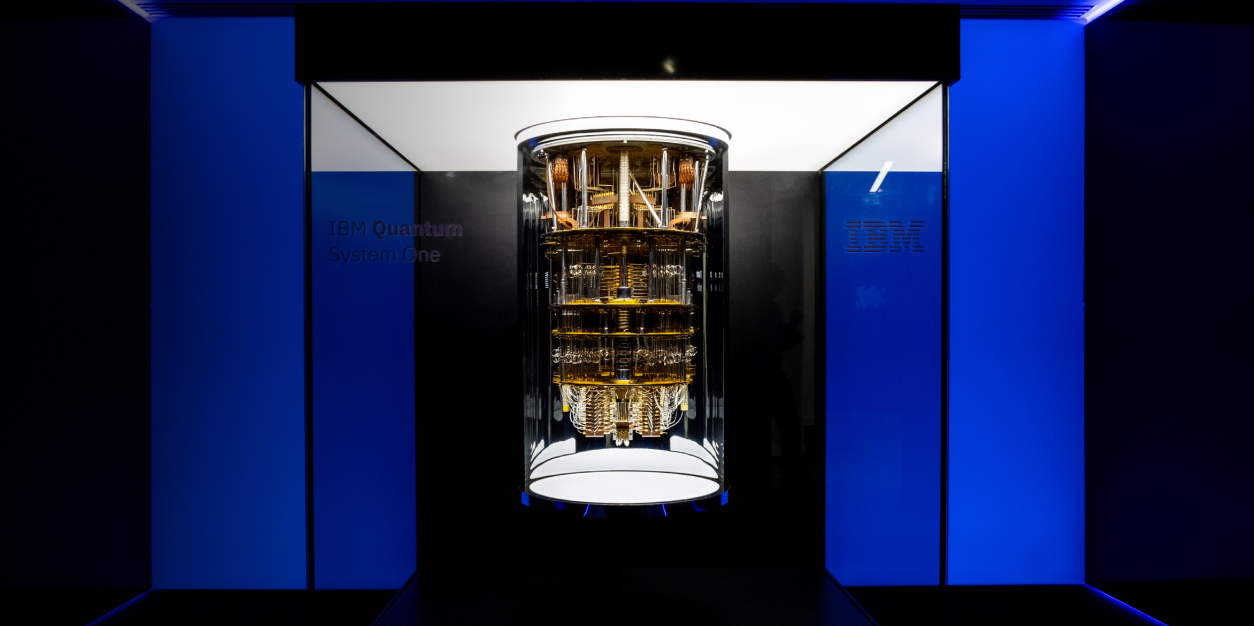
\includegraphics[width=0.7\linewidth]{SystemOne}
	\caption{IBM Q System One}
	\label{fig:systemone}
\end{figure}


\section{Veszélyek}

\section{Lehetőségek}

\chapter{Klasszikus- és kvantum logikai kapuk}
\section{Klasszikus logikai kapuk és áramkörök}
Elektromos impulzusokhoz értékeket társítunk, az alapján hogy küldtünk-e vagy sem. Ha érzékelünk, akkor ezt I logikai értéknek vagy 1 bitnek tekintjük. Ellenkező esetben H logikai értéknek, vagy 0 bitnek feleltetjük meg.

Ezekhez az impulzusokhoz többnyire logikai kapukat társítunk, melyek bináris operátorokat foglalnak magukban. A logikai kapuk alapvető építőkövei az elektronikának és számos célra használják őket. Összekapcsolásukkal áramköröket alakíthatunk ki, amik lineárisak és balról jobbra értelmezzük őket. A bal oldali vezetékek jelentik a bemenetet, míg a jobb oldaliak a kimenetet. Az ismertebb kapukhoz speciális ábrák és igazságtáblák tartoznak.

Az igazságtáblák a klasszikus logika alapvető eszközei, amelyek segítségével értelmezhetjük az adott műveleteket, valamint ellenőrizhetjük áramköreinket. Megmutatják az összes lehetséges bemeneti kombinációt, illetve a műveletek alkalmazása után a várható kimenetet is. Ezek a logikai műveleteket, kifejezéseket Boole-algebrának nevezzük, amely egy 19. századi matematikus, George Boole nevét viseli
\subsection{Logikai kapuk}
\subsubsection{Buffer}
A buffer kapuk kimenete megegyezik a kimenetükkel, egy biten értelmezzük. Jele: $A$

\begin{figure}[H]
	\centering
	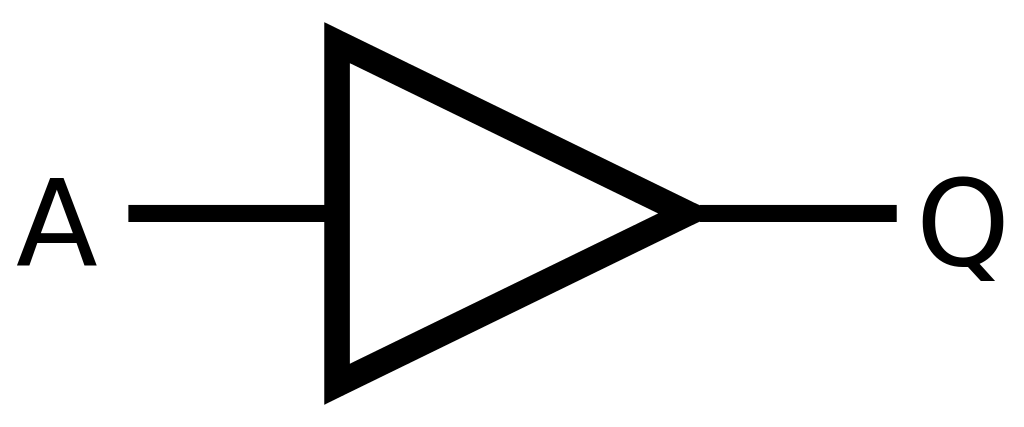
\includegraphics[width=0.3\linewidth]{buffer}
	\caption{Buffer kapu rajza}
	\label{fig:buffer}
\end{figure}


\begin{table}[H]
	\centering
	\begin{tabular}{c|c}
		$A$ & $A$\\
		\hline
		0 & 0\\
		1 & 1
	\end{tabular}
	\caption{Buffer kapu igazságtáblája}
\end{table}

\subsubsection{NOT, vagy Negáció}
A negáció kapu (vagy NOT) hasonlóan egy bites, a bemeneti jel logikai értékét megfordítja a kimeneten. Jele:$\neg A$

\begin{figure}[H]
	\centering
	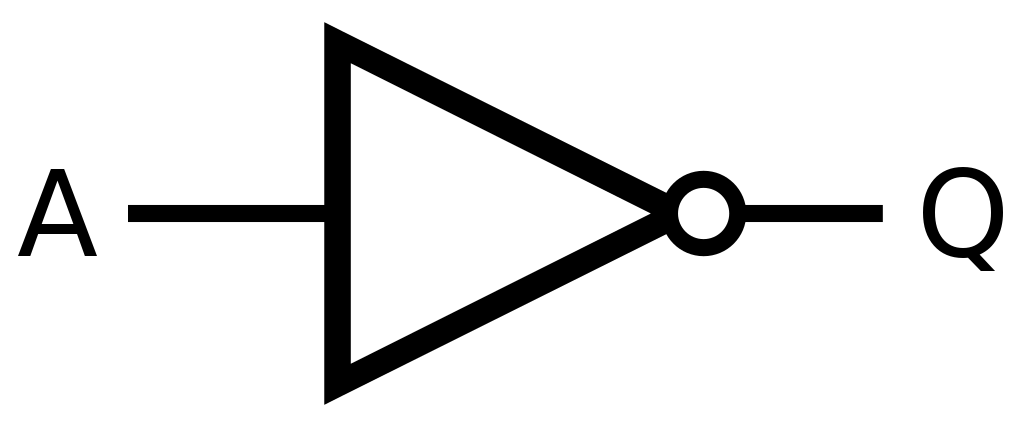
\includegraphics[width=0.3\linewidth]{not}
	\caption{NOT kapu rajza}
	\label{fig:not}
\end{figure}


\begin{table}[H]
	\centering
	\begin{tabular}{c|c}
		$A$ & $\neg A$\\
		\hline
		0 & 1\\
		1 & 0 
	\end{tabular}
	\caption{Negáció kapu igazságtáblája}
\end{table}

\subsubsection{AND, vagy Konjukció}
Más néven logikai és. Kétbites művelet, kimenete akkor igaz, ha mind a két operandusa igaz. Jele: $A \land B$

\begin{figure}[H]
	\centering
	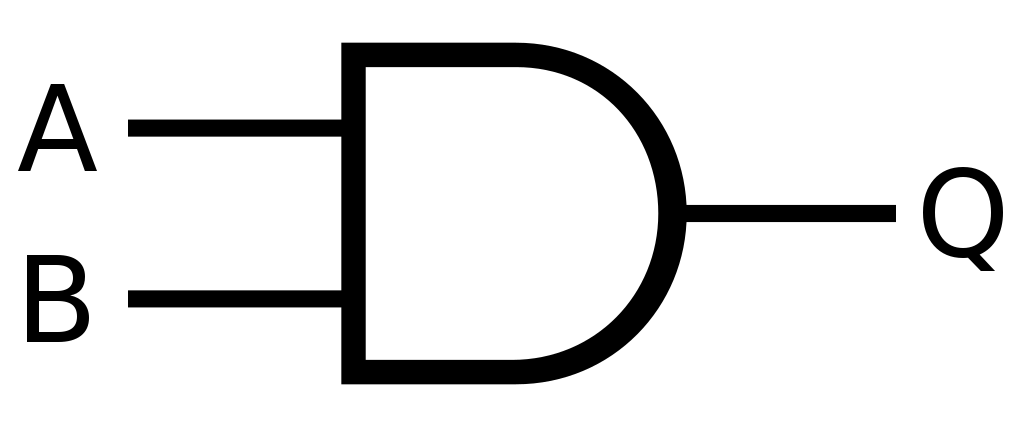
\includegraphics[width=0.3\linewidth]{and}
	\caption{AND kapu rajza}
	\label{fig:and}
\end{figure}


\begin{table}[H]
	\centering
	\begin{tabular}{c|c|c}
		$A$ & $B$ & $A \land B$\\               
		\hline
		0 & 0 & 0\\
		0 & 1 & 0\\
		1 & 0 & 0\\
		1 & 1 & 1
	\end{tabular}
	\caption{A konjukció igazságtáblája}
\end{table}

\subsubsection{OR, vagy Diszjunkció}
Más néven logikai vagy. Szintén kétbites művelet, értéke csak akkor hamis, ha mind a két operandusa hamis. Jele: $A \lor B$

\begin{figure}[H]
	\centering
	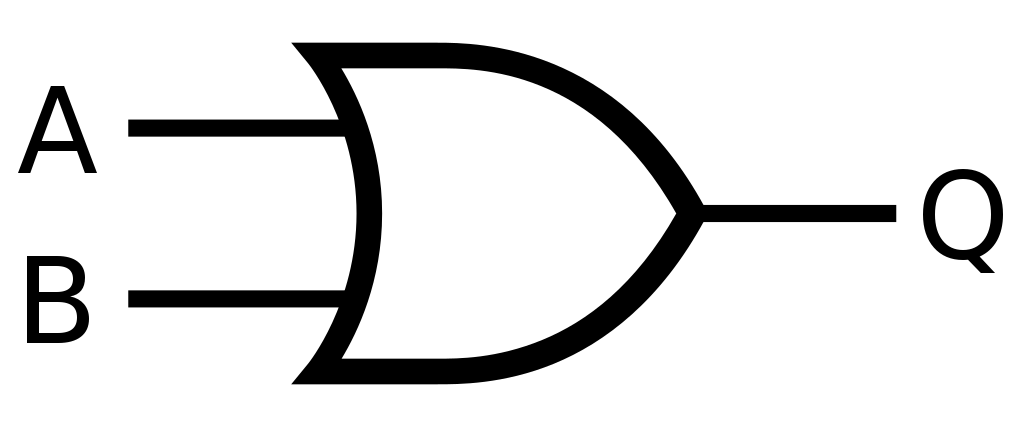
\includegraphics[width=0.3\linewidth]{or}
	\caption{OR kapu rajza}
	\label{fig:or}
\end{figure}


\begin{table}[H]
	\centering
	\begin{tabular}{c|c|c}
		$A$ & $B$ & $A \lor B$\\               
		\hline
		0 & 0 & 0\\
		0 & 1 & 1\\
		1 & 0 & 1\\
		1 & 1 & 1
	\end{tabular}
	\caption{A diszjunkció igazságtáblája}
\end{table}

\subsubsection{NAND, vagy Negált konjukció}
A konjukció negált változata, értéke akkor hamis, ha mindkét operandusa igaz. Jele: $\neg(A \land B)$

\begin{figure}[H]
	\centering
	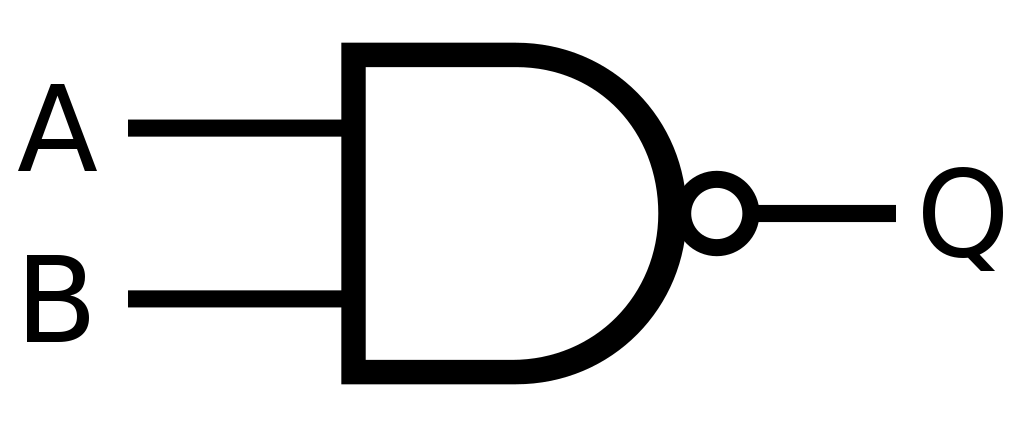
\includegraphics[width=0.3\linewidth]{nand}
	\caption{NAND kapu rajza}
	\label{fig:nand}
\end{figure}


\begin{table}[H]
	\centering
	\begin{tabular}{c|c|c}
		$A$ & $B$ & $\neg(A \land B)$\\               
		\hline
		0 & 0 & 1\\
		0 & 1 & 1\\
		1 & 0 & 1\\
		1 & 1 & 0
	\end{tabular}
	\caption{A negált konjukció igazságtáblája}
\end{table}

\subsubsection{NOR, vagy Negált diszjunkció}
A diszjunkció negált változata, értéke akkor igaz, ha mindkét operandusa hamis. Jele: $\neg(A \lor B)$

\begin{figure}[H]
	\centering
	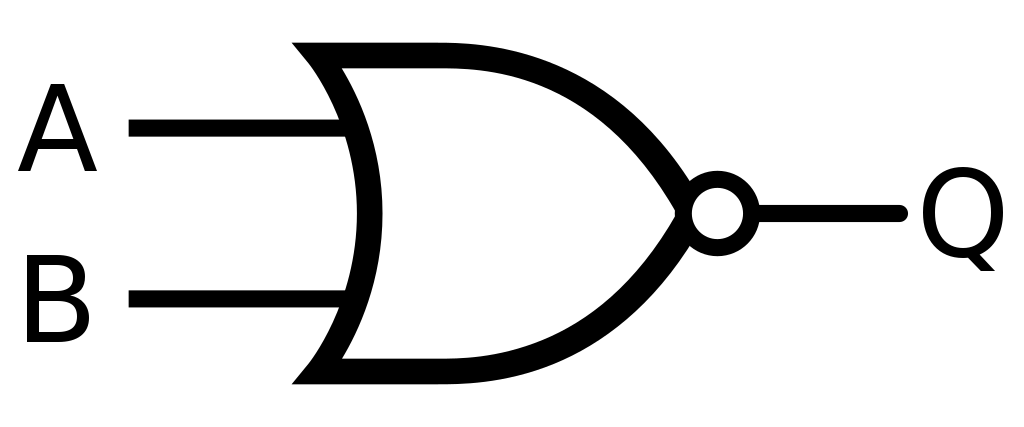
\includegraphics[width=0.3\linewidth]{nor}
	\caption{NOR kapu rajza}
	\label{fig:nor}
\end{figure}


\begin{table}[H]
	\centering
	\begin{tabular}{c|c|c}
		$A$ & $B$ & $\neg(A \lor B)$\\               
		\hline
		0 & 0 & 1\\
		0 & 1 & 0\\
		1 & 0 & 0\\
		1 & 1 & 0
	\end{tabular}
	\caption{A negált diszjunkció igazságtáblája}
\end{table}


\subsubsection{XOR, vagy Exclusive OR}
Más néven kizáró vagy. Értéke akkor hamis, ha a bemenetek megegyeznek. Jele: $A \oplus B$

\begin{figure}[H]
	\centering
	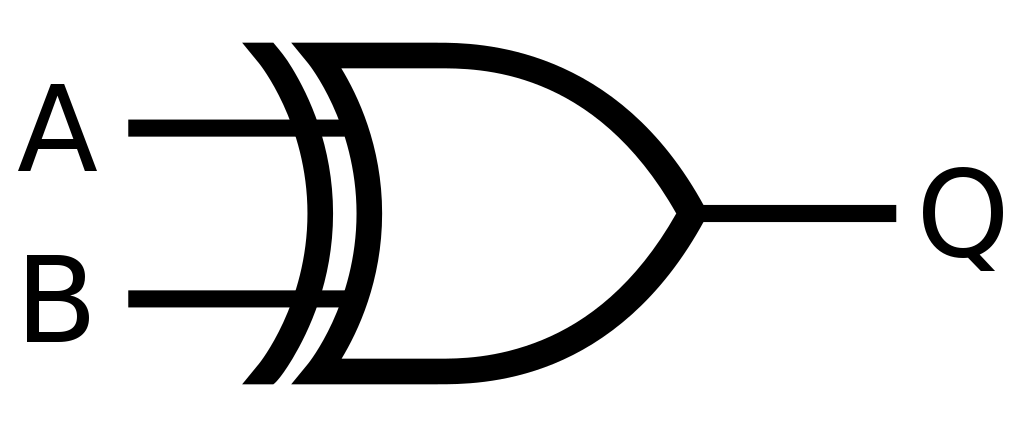
\includegraphics[width=0.3\linewidth]{xor}
	\caption{XOR kapu rajza}
	\label{fig:xor}
\end{figure}


\begin{table}[H]
	\centering
	\begin{tabular}{c|c|c}
		$A$ & $B$ & $A \oplus B$\\               
		\hline
		0 & 0 & 0\\
		0 & 1 & 1\\
		1 & 0 & 1\\
		1 & 1 & 0
	\end{tabular}
	\caption{A negált konjukció igazságtáblája}
\end{table}


\subsubsection{XNOR, vagy Exclusive NOR}
A kizáró vagy negáltja, értéke akkor hamis, ha a bemenetek különböznek Jele: $\neg (A \oplus B)$

\begin{figure}[H]
	\centering
	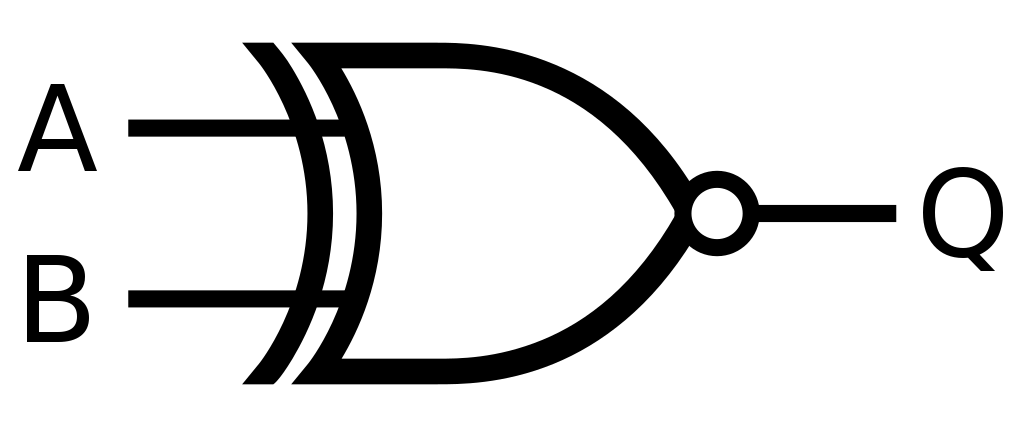
\includegraphics[width=0.3\linewidth]{xnor}
	\caption{XNOR kapu rajza}
	\label{fig:xnor}
\end{figure}


\begin{table}[H]
	\centering
	\begin{tabular}{c|c|c}
		$A$ & $B$ & $\neg (A \oplus B)$\\               
		\hline
		0 & 0 & 1\\
		0 & 1 & 0\\
		1 & 0 & 0\\
		1 & 1 & 1
	\end{tabular}
	\caption{A negált konjukció igazságtáblája}
\end{table}

\subsection{Univerzális kapuk}
Léteznek olyan logikai kapuk, amelyek képesek reprodukálni bármely másik működését. Ezek az univerzális kapuk lehetővé teszik akármelyik logikai függvény leképezését, ami azt jelenti, hogy akár tetszőleges áramkör is megvalósítható velük.

Bizonyítható, hogy bármilyen logikai függvény összeállítható csak NOT és AND, vagy NOT és OR függvények kombinációival. Mint láttuk, ezek a kapuk ötvözhetőek, erre szolgálnak a NAND és NOR kapuk.

Ebből következtethető, hogy bármilyen Boole-függvény megvalósítható olyan áramkörrel, amely csak NAND vagy NOR kapukat alkalmaz. Gyakran emiatt előnyt élveznek, mivel más kapuknak nincs ilyen tulajdonsága.

\section{Kvantum logikai kapuk és áramkörök}
A kvantumkapuk jelentőségét a kvantummechanika alapelveire támaszkodva értelmezhetjük, amelyek olyan jelenségeket és viselkedéseket írnak le, melyek a klasszikus fizika keretein belül nem megfigyelhetők vagy magyarázhatók. A kvantummechanika alapján működő kapuk és áramkörök lehetővé teszik olyan számítások végrehajtását, amelyek rendkívül nagy számítási kapacitással és párhuzamosítással rendelkeznek, ami jelentős előnyöket kínál a hagyományos, klasszikus számítógépekkel szemben.

Bár vannak hasonlóságok a klasszikus változatokhoz képest, a kvantum logikai kapuk egy sokkal komplexebb matematikai hátteret és fizikai jelenségeket hordoznak magukban.

Jelen alfejezet csak pár, ismertebb logikai kaput tartalmaz, de fontos megemlíteni, hogy a kvantumkapuk száma végtelen. Mivel szakdolgozatom az egyqubites kapukra irányul, ezért a több kvantumbites változatok csak megemlítő jelleggel szerepelnek.

\subsection{Qubit}
A kvantumbit, röviden qubit, a kvantuminformatika alapvető építőeleme, és a klasszikus számítógépek működésétől eltérő, kvantummechanikai alapokon nyugvó adatábrázolási egység. Míg a hagyományos bit csak két állapotban (0 vagy 1) lehet jelen, a qubit képes egyszerre számos állapotban lenni, ami egyike annak a tulajdonságának, amely a kvantuminformatikát annyira különlegessé teszi.

\begin{figure}[H]
	\centering
	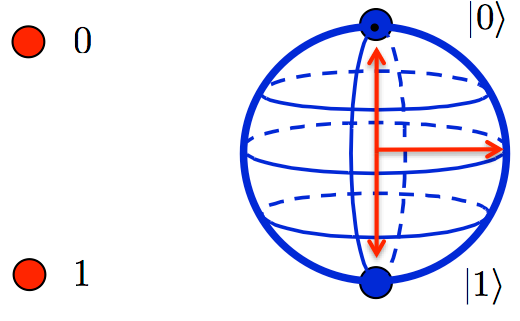
\includegraphics[width=0.3\linewidth]{bitQubit}
	\caption{A bit és qubit reprezentációja}
	\label{fig:bitqubit}
\end{figure}

Ahogy az \az{\ref{fig:bitqubit}}.~ábrán látható, a qubit számos állapotát egy úgynevezett Bloch gömbön ábrázoljuk, északi pólusán $\ket{0}$, déli pólusán pedig $\ket{1}$ helyezkedik el. A $\ket{}$ és $\bra{}$ jelöléseket braket-nek nevezzük, de Dirac jelölésként is ismert, és a kvantumállapotok jelölésében segít. A ket ($\ket{\Psi}$) egy oszlopvektort, a bra ($\bra{\Psi}$) pedig egy sorvektort jelöl.

A kvantummechanika alapelvei és a qubitok sajátos tulajdonságai lehetővé teszik
olyan számítási feladatok elvégzését, amelyek a hagyományos számítógépek számára gyakorlatilag lehetetlenek lennének.

\subsection{Szuperpozíció és összefonódás}

Egy qubit állapotát a következőképpen adhatjuk meg:
\begin{equation}
	\ket{\Psi}=\alpha\ket{0}+\beta\ket{1},
\end{equation}
ahol $\alpha$ és $\beta$ komplex számok, valamint teljesül, hogy $|\alpha|^2+|\beta|^2=1$. Ez azt jelenti, hogy a $\ket{\Psi}$ kvantumbit $|\alpha|^2$ eséllyel 0, $|\beta|^2$-el pedig 1 lesz. Ezt szuperpozíciónak nevezzük. A két szélső érték, azaz $\ket{0}$ vagy $\ket{1}$ akkor áll elő, ha $\alpha$ 0 vagy 1, $\beta$ pedig ennek ellentettje. A szuperpozíció legjobban a Schrödinger macskája gondolatkísérlettel prezentálható, melyet Erwin Schrödinger fogalmazott meg 1935-ben.

A qubit másik fontos jelensége a kvantum-összefonódás. Ez egy olyan jelenség a kvantummechanikában, amelyben két vagy több részecske állapota olyan összekapcsolt módon van, hogy az egyiken végzett mérések azonnal hatnak a másikra, függetlenül attól, hogy a részecskék milyen fizikai távolságra vannak egymástól.

\subsection{Qubit mérése}
Méréskor eredményként egyetlen klasszikus bitet kapunk. A qubit mérése során az eredmény kvantumállapota "összeomlik" az adott értékre, amelyet a mérés során megfigyeltünk. Azaz elveszti a szuperpozícióját és az összefonódottságát, ami azt jelenti, hogy a mérés után a rendszer elveszíti a kvantumos jellegét, és klasszikus állapotba kerül. Ez az összeomlás a kvantummechanika alapvető jelensége, amely lehetővé teszi a kvantumrendszer állapotának rögzítését a mérés pillanatában. Emiatt a mérések kritikus szerepet játszanak.

\begin{figure}[H]
	\centering
	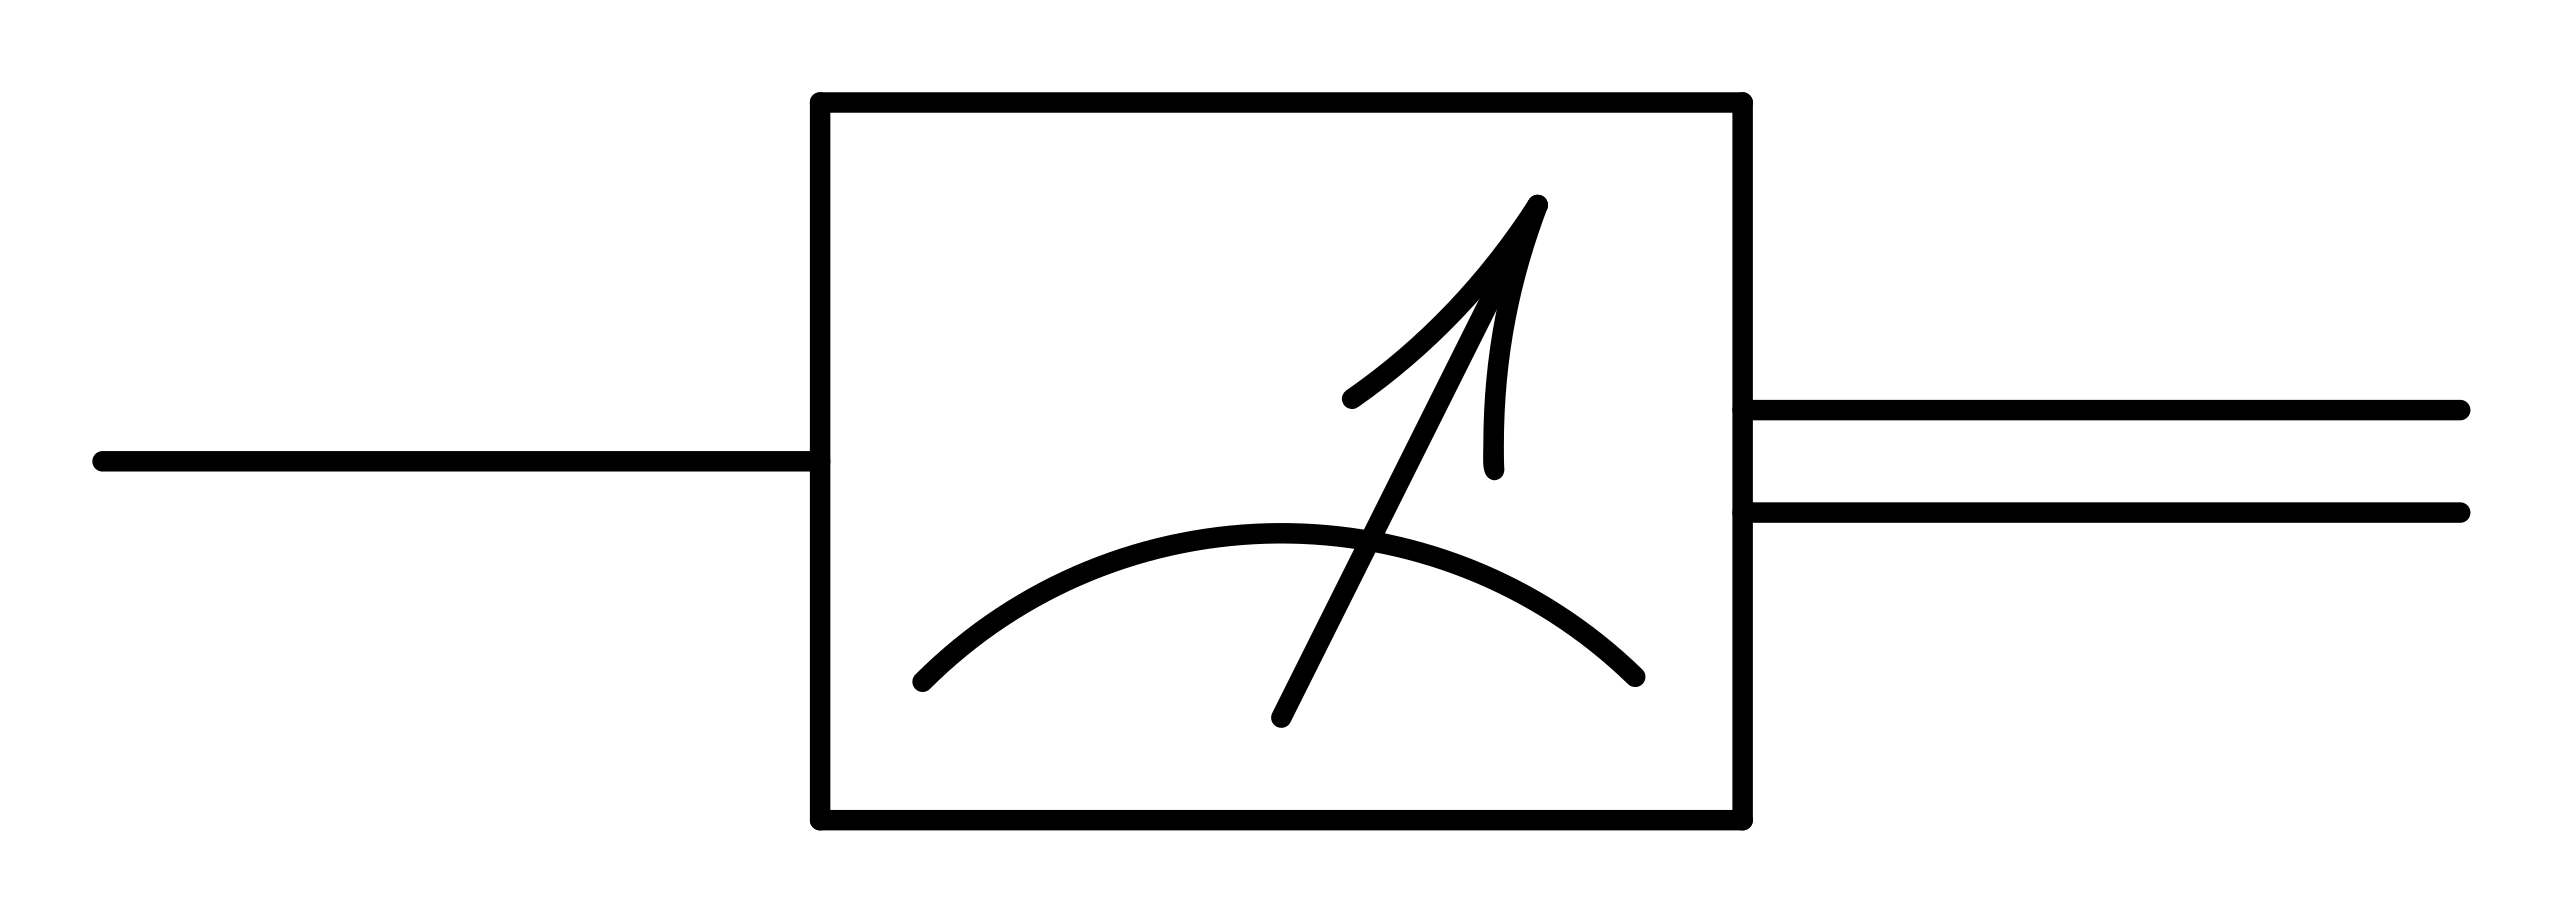
\includegraphics[width=0.3\linewidth]{measure}
	\caption{Mérés rajza}
	\label{fig:measure}
\end{figure}

\subsection{Kvantum logikai kapuk}\label{kvantumkapuk}

\subsubsection{I, vagy Identity}
A buffer kapuhoz hasonlóan nem végez műveletet, helyben hagyja a kvantumbiteket. Egy qubiten használjuk. Azonosság transzformációként működik, alakja:

\begin{equation}
	I= 
	\begin{bmatrix}
		1 & 0\\
		0 & 1
	\end{bmatrix}
\end{equation}

Ez egy tetszőleges kvantumbiten:

\begin{equation}
	\ket{\Psi}=I\ket{\varphi}
		\begin{bmatrix}
			1 & 0\\
			0 & 1
		\end{bmatrix}
		\begin{bmatrix}
			a\\
			b
		\end{bmatrix}=a\ket{0}+b\ket{1}
\end{equation}


\begin{figure}[H]
	\centering
	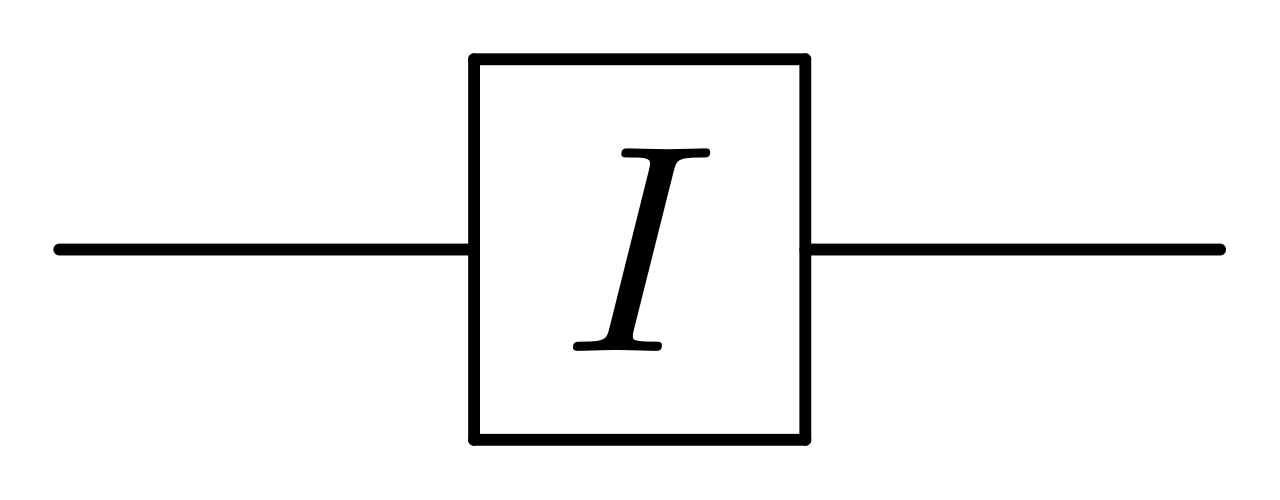
\includegraphics[width=0.3\linewidth]{Identity}
	\caption{I kapu rajza}
	\label{fig:identity}
\end{figure}


\subsubsection{X, vagy Pauli-X}
A klasszikus NOT kapunak felel meg, bit-flipnek is hívják. A Bloch gömb $X$ tengelyére tükröz. Egy qubiten működik. Alakja:

\begin{equation}
	X= 
	\begin{bmatrix}
		0 & 1\\
		1 & 0
	\end{bmatrix}
\end{equation}

Ez egy tetszőleges kvantumbiten:

\begin{equation}
	\ket{\Psi}=X\ket{\varphi}
		\begin{bmatrix}
			0 & 1\\
			1 & 0
		\end{bmatrix}
		\begin{bmatrix}
			a\\
			b
		\end{bmatrix}=b\ket{0}+a\ket{1}
\end{equation}


Az X kapu hatására a valószínűségi amplitúdók cserélődnek. Inverze saját maga, tehát például:

\begin{equation}
	\ket{\Psi}=XX\ket{0}=\ket{0}
\end{equation}

\begin{figure}[H]
	\centering
	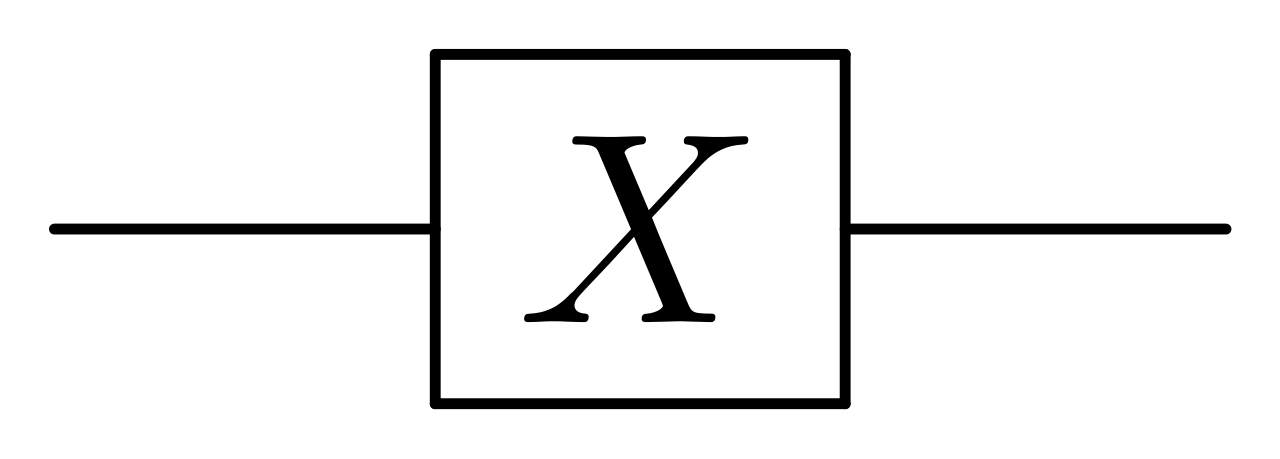
\includegraphics[width=0.3\linewidth]{Pauli_X}
	\caption{X kapu rajza}
	\label{fig:paulix}
\end{figure}


\subsubsection{Y, vagy Pauli-Y}
Az X kapuhoz hasonlóan felcseréli a $\ket{0}$-t és az $\ket{1}$-t, viszont az Y kapu a relatív fázist is megváltoztatja. A Bloch gömb $Y$ tengelyére tükröz. Egy qubiten működik. Alakja:

\begin{equation}
	Y= 
	\begin{bmatrix}
		0 & -i\\
		i & 0
	\end{bmatrix}
\end{equation}

Ez egy tetszőleges kvantumbiten:

\begin{equation}
	\ket{\Psi}=Y\ket{\varphi}
		\begin{bmatrix}
			0 & -i\\
			i & 0
		\end{bmatrix}
		\begin{bmatrix}
			a\\
			b
		\end{bmatrix}=-ib\ket{0}+ia\ket{1},
\end{equation}

ahol $i$ komplex szám. Inverze saját maga, tehát például:

\begin{equation}
	\ket{\Psi}=YY\ket{0}=\ket{0}
\end{equation}

\begin{figure}[H]
	\centering
	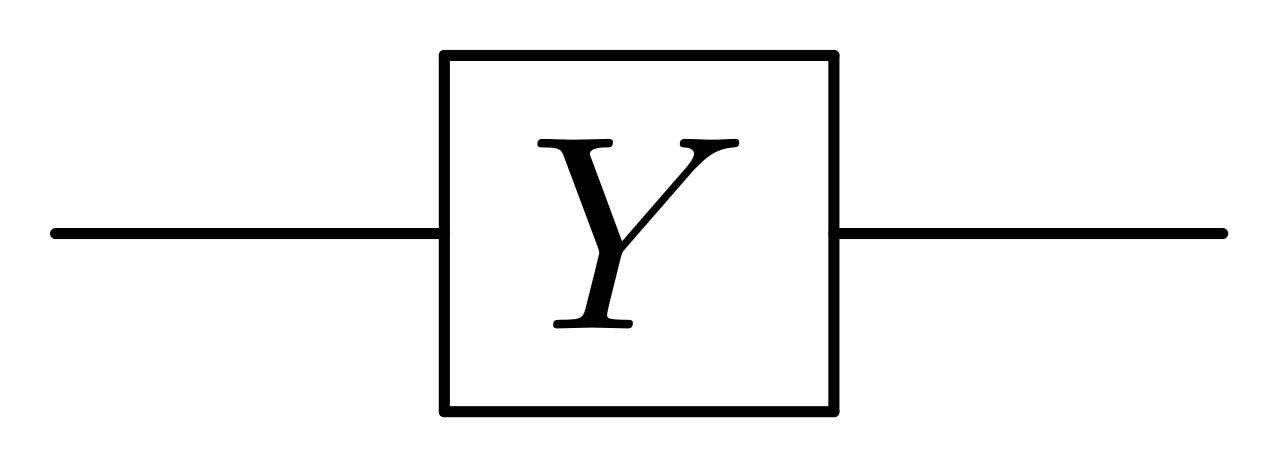
\includegraphics[width=0.3\linewidth]{Pauli_Y}
	\caption{Y kapu rajza}
	\label{fig:pauliy}
\end{figure}


\subsubsection{Z, vagy Pauli-Z}
Phase-flip kapunak is hívják, ebből adódóan a fázist cseréli meg. A Bloch gömb $Z$ tengelyére tükröz. Egy qubiten működik. Alakja:

\begin{equation}
	Z= 
	\begin{bmatrix}
		1 & 0\\
		0 & -1
	\end{bmatrix}
\end{equation}

Ez egy tetszőleges kvantumbiten:

\begin{equation}
	\ket{\Psi}=Z\ket{\varphi}
		\begin{bmatrix}
			1 & 0\\
			0 & -1
		\end{bmatrix}
		\begin{bmatrix}
			a\\
			b
		\end{bmatrix}=a\ket{0}-b\ket{1}
\end{equation}

Látható, hogy a Z kapu csak az $\ket{1}$ valószínűségi amplitúdót változtatja. Inverze saját maga, tehát például:

\begin{equation}
	\ket{\Psi}=ZZ\ket{0}=\ket{0}
\end{equation}

\begin{figure}[H]
	\centering
	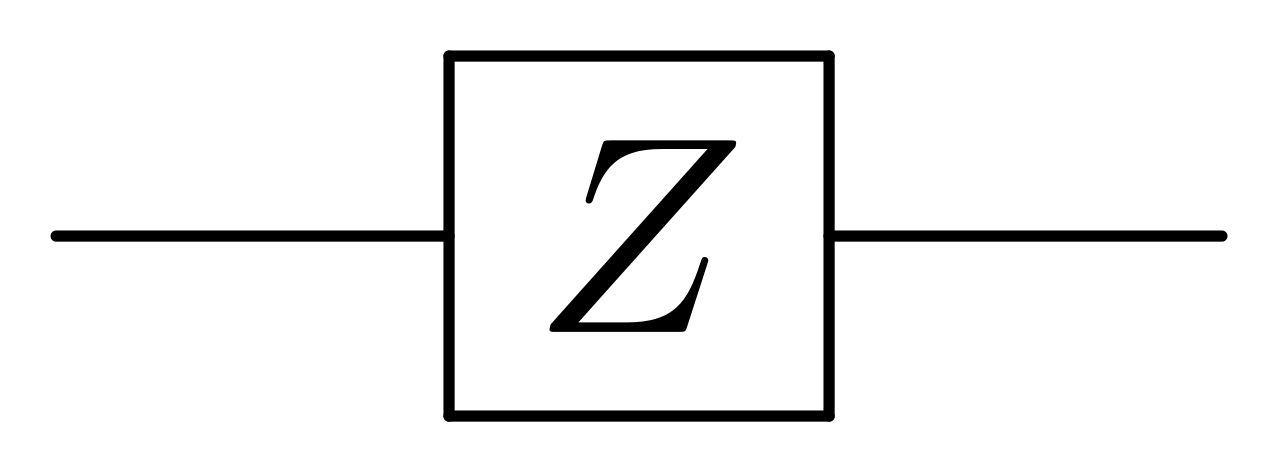
\includegraphics[width=0.3\linewidth]{Pauli_Z}
	\caption{Z kapu rajza}
	\label{fig:pauliz}
\end{figure}

\subsubsection{H, vagy Hadamard}
A Hadamard kapu segítségével a már említett szuperpozíciós állapotokat lehet előállítani. Egy qubiten működik. Alakja:

\begin{equation}
	H= \frac{1}{\sqrt{2}}
	\begin{bmatrix}
		1 & 1\\
		1 & -1
	\end{bmatrix}
\end{equation}

Ez egy tetszőleges kvantumbiten:

\begin{equation}
	\ket{\Psi}=H\ket{\varphi}=\frac{1}{\sqrt{2}}
	\begin{bmatrix}
		1 & 1\\
		1 & -1
	\end{bmatrix}
	\begin{bmatrix}
		a\\
		b
	\end{bmatrix}=\frac{a+b}{\sqrt{2}}\ket{0}+\frac{a-b}{\sqrt{2}}\ket{1}
\end{equation}

Mivel a kaput gyakran használják a standard bázisvektorokon, emiatt külön számon tartják őket:

\begin{equation}
	\ket{\Psi}=H\ket{0}=\frac{1}{\sqrt{2}}
	\begin{bmatrix}
		1 & 1\\
		1 & -1
	\end{bmatrix}
	\begin{bmatrix}
		1\\
		0
	\end{bmatrix}=\frac{\ket{0}+\ket{1}}{\sqrt{2}}
\end{equation}

\begin{equation}
	\ket{\Psi}=H\ket{1}=\frac{1}{\sqrt{2}}
	\begin{bmatrix}
		1 & 1\\
		1 & -1
	\end{bmatrix}
	\begin{bmatrix}
		0\\
		1
	\end{bmatrix}=\frac{\ket{0}-\ket{1}}{\sqrt{2}}
\end{equation}

A Hadamard kapu inverze saját maga, tehát például:

\begin{equation}
	\ket{\Psi}=HH\ket{0}=\ket{0}
\end{equation}

\begin{figure}[H]
	\centering
	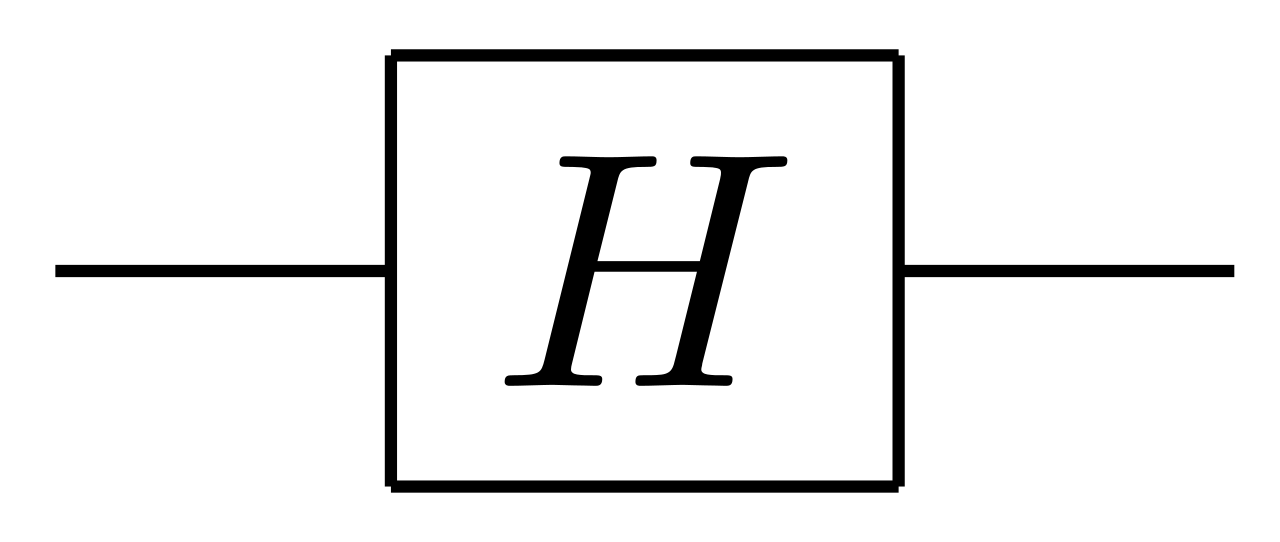
\includegraphics[width=0.3\linewidth]{Hadamard}
	\caption{H kapu rajza}
	\label{fig:hadamard}
\end{figure}


\subsubsection{S, vagy Phase}
Más néven fáziseltolási kapu. $\pi/2$ fáziseltolást alkalmaz a qubit állapotára. A Bloch gömb körül az óramutató járásával megegyező irányban forgat $\pi/2$ radiánnal. Egy qubiten működik. Alakja:

\begin{equation}
	S= 
	\begin{bmatrix}
		1 & 0\\
		0 & -i
	\end{bmatrix}
\end{equation}

Ez egy tetszőleges kvantumbiten:

\begin{equation}
	\ket{\Psi}=S\ket{\varphi}=
	\begin{bmatrix}
		1 & 0\\
		0 & -i
	\end{bmatrix}
	\begin{bmatrix}
		a\\
		b
	\end{bmatrix}=a\ket{0}-ib\ket{1}
\end{equation}

\begin{figure}[H]
	\centering
	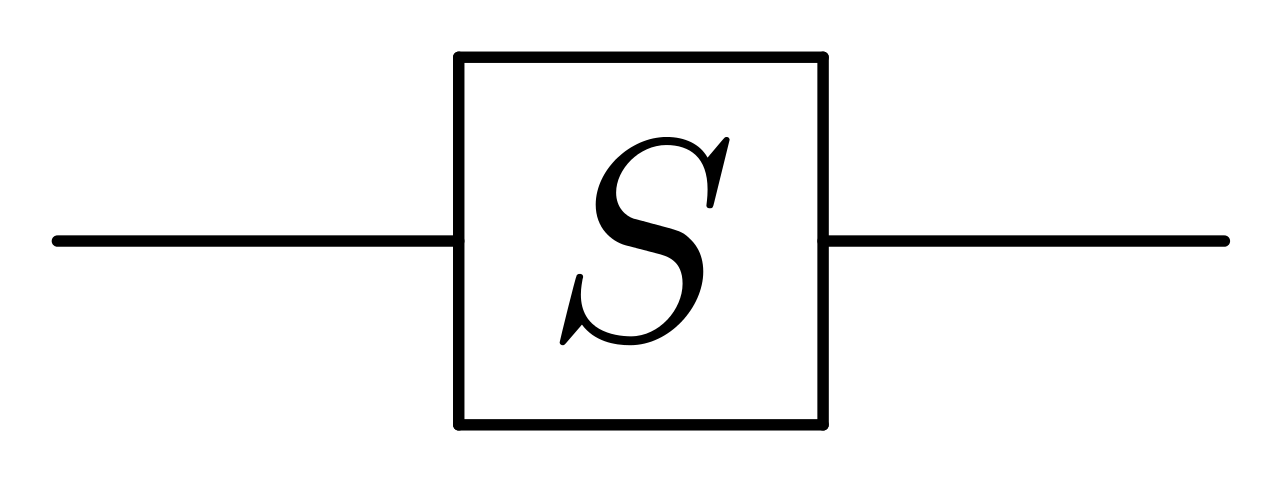
\includegraphics[width=0.3\linewidth]{Qcircuit_S.svg}
	\caption{S kapu rajza}
	\label{fig:qcircuits}
\end{figure}


\subsubsection{T, vagy $\pi/8$}
A T kapu, hasonlóan az S kapuhoz, fáziseltolást alkalmaz egy qubit állapotára. Az állapotvektort $\pi/4$ radiánnal forgat a Bloch gömb körül, óramutató járással megegyező irányban. Alakja:

\begin{equation}
	T= 
	\begin{bmatrix}
		1 & 0\\
		0 & e^{i\pi/4}
	\end{bmatrix}
\end{equation}

Ez egy tetszőleges kvantumbiten:

\begin{equation}
	\ket{\Psi}=T\ket{\varphi}=
	\begin{bmatrix}
		1 & 0\\
		0 & e^{i\pi/4}
	\end{bmatrix}
	\begin{bmatrix}
		a\\
		b
	\end{bmatrix}=a\ket{0}+e^{i\pi/4}b\ket{1}
\end{equation}

Az S kapuval való azonosságok miatt elmondható, hogy $S=T^{2}$

\begin{figure}[H]
	\centering
	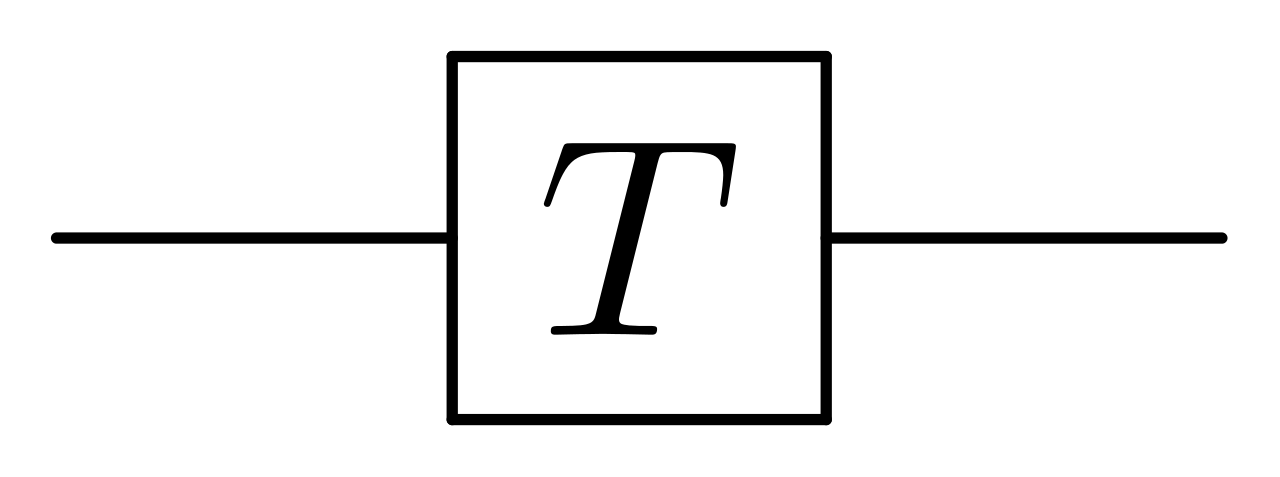
\includegraphics[width=0.3\linewidth]{Qcircuit_T.svg}
	\caption{T kapu rajza}
	\label{fig:qcircuitt}
\end{figure}


\subsubsection{CNOT, vagy Controlled Not}
A CNOT kapu két qubites művelet, ahol az első qubit vezérlő-, a második pedig cél kvantumbit néven ismert. Ha a vezérlő $\ket{1}$, akkor a cél qubiten X kaput használ, a többi változatlan. Amennyiben a vezérlő qubit $\ket{0}$, a cél változatlan marad. Klasszikus logikai kapuként is alkalmazható. Inverze saját maga. Alakja:

\begin{equation}
	CNOT= 
	\begin{bmatrix}
		1 & 0 & 0 & 0\\
		0 & 1 & 0 & 0\\
		0 & 0 & 0 & 1\\
		0 & 0 & 1 & 0
	\end{bmatrix}
\end{equation}

\begin{figure}[H]
	\centering
	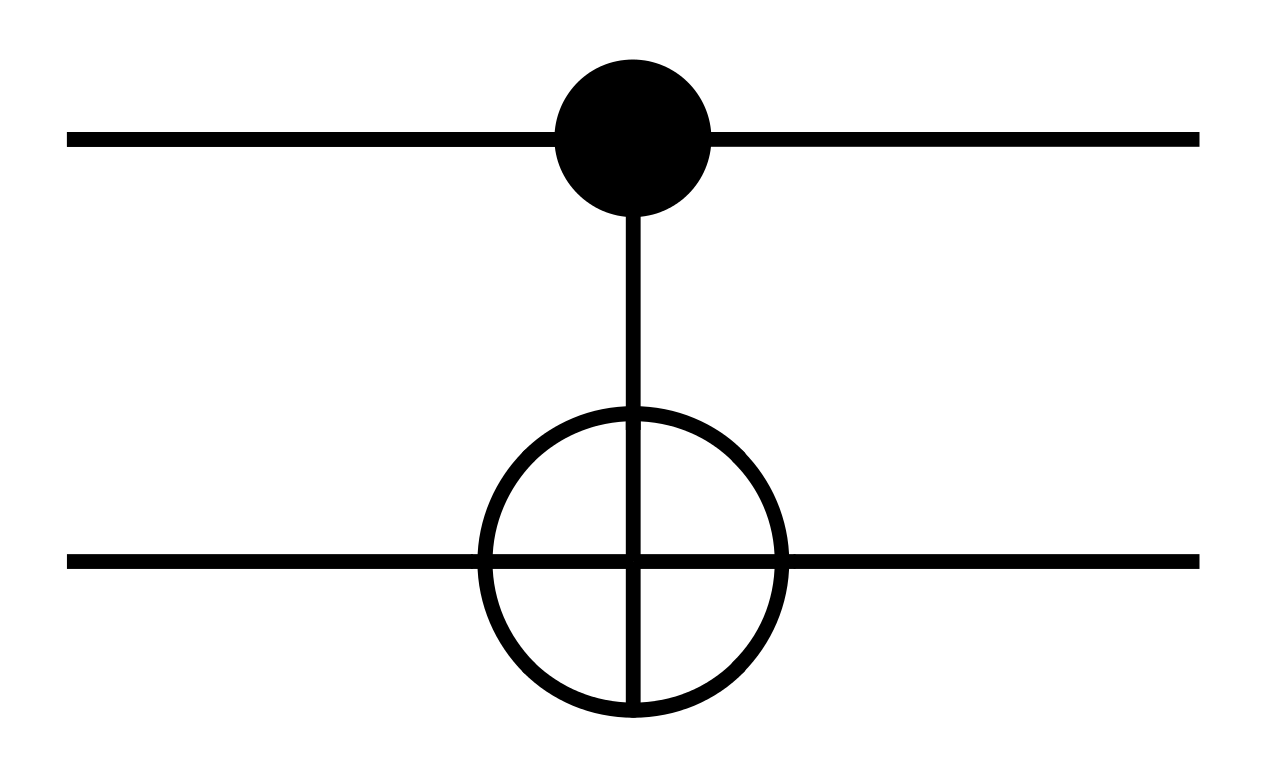
\includegraphics[width=0.25\linewidth]{CNOT}
	\caption{CNOT kapu rajza}
	\label{fig:cnot}
\end{figure}


\subsubsection{SWAP}
Két qubites kvantumkapu, mely felcseréli a bemenetek állapotát. Mivel három CNOT kapuval valósítható meg, így más jelölést is alkalmaznak rá, az egyszerűbb változat \az{\ref{fig:swap}}.~ábrán látható. Inverze saját maga. Alakja:

\begin{equation}
	SWAP= 
	\begin{bmatrix}
		1 & 0 & 0 & 0\\
		0 & 0 & 1 & 0\\
		0 & 1 & 0 & 0\\
		0 & 0 & 0 & 1
	\end{bmatrix}
\end{equation}

\begin{figure}[H]
	\centering
	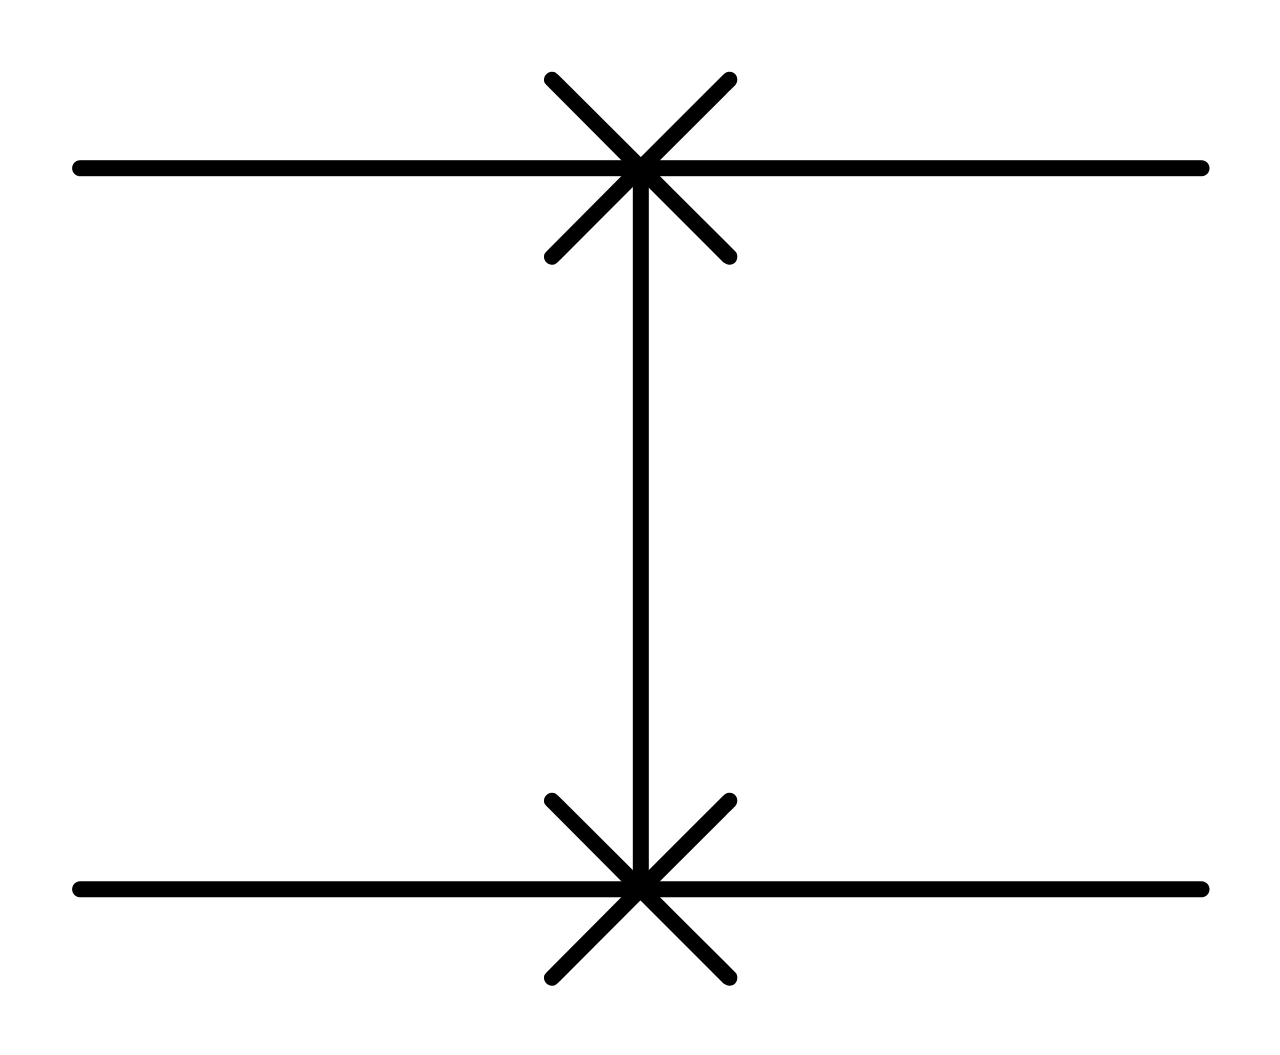
\includegraphics[width=0.25\linewidth]{SWAP}
	\caption{SWAP kapu rajza}
	\label{fig:swap}
\end{figure}


\subsubsection{Toffoli}
Ahogy az \az{\ref{fig:toffoligate}}.~ábrán látható, a Toffoli kapu CNOT műveletet használ, ezért szokás CCNOT kapunak is nevezni. Három qubiten működik, az első kettő vezérlő, az utolsó pedig a cél qubit. Klasszikus logikai kapuként is alkalmazható, ez esetben univerzális klasszikus kapunak tekintik. Inverze saját maga. Alakja:

\begin{equation}
	Toffoli= 
	\begin{bmatrix}
		1 & 0 & 0 & 0 & 0 & 0 & 0 & 0\\
		0 & 1 & 0 & 0 & 0 & 0 & 0 & 0\\
		0 & 0 & 1 & 0 & 0 & 0 & 0 & 0\\
		0 & 0 & 0 & 1 & 0 & 0 & 0 & 0\\
		0 & 0 & 0 & 0 & 1 & 0 & 0 & 0\\
		0 & 0 & 0 & 0 & 0 & 1 & 0 & 0\\
		0 & 0 & 0 & 0 & 0 & 0 & 0 & 1\\
		0 & 0 & 0 & 0 & 0 & 0 & 1 & 0\\
	\end{bmatrix}
\end{equation}

\begin{figure}[H]
	\centering
	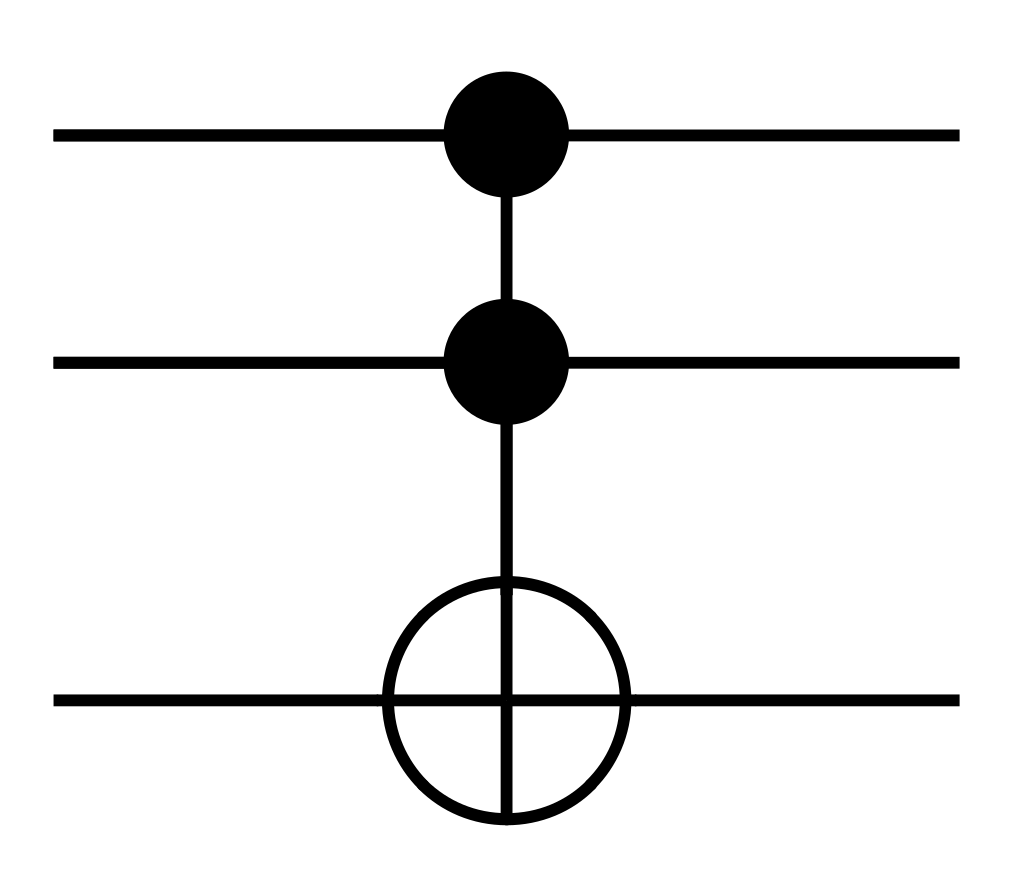
\includegraphics[width=0.25\linewidth]{Toffoli_gate.svg}
	\caption{Toffoli kapu rajza}
	\label{fig:toffoligate}
\end{figure}


\subsection{Univerzális kvantumkapuk}
Klasszikus esetben tapasztaltuk, hogy léteznek univerzális kapuk. Ez amiatt lehetséges, mivel csak végesen sok Boole-függvény van egy adott számú változó esetén. Kvantumkapuknál elmondható, hogy a lehetséges kapuk száma végtelen sok. Emiatt a fontos különbség miatt univerzális kvantumkapuk halmaza sem létezik. Ellenben, ha a kapuknak vesszük egy véges számú gyűjteményét, akkor beszélhetünk univerzális megoldásokról, viszont ezek sem használhatóak minden lehetséges kvantumáramkörre, csak hozzávetőlegesen.

\section{Reverzibilis kapuk}
Megfordítható kapuknak is nevezik őket. Két alapvető tulajdonsága van:
\begin{enumerate}
	\item Az eredményükből egyértelműen kikövetkeztethetőek a bemenetek, azaz egy bemeneti kombinációhoz pontosan egy kimeneti kombináció tartozik, és fordítva
	\item Lehetővé teszik a bemenetek helyreállítását a kimenetekből anélkül, hogy információt veszítenének.
\end{enumerate}

Vegyük például az OR kaput. Mint láttuk, értéke csak akkor hamis, ha bemenetei hamisak. Viszont minden más esetben nem tudjuk megállapítani, hogy melyik volt az aktuális bemenet a háromból, hacsak nincs további információnk. Tehát az OR kapuról elmondható, hogy irreverzibilis (nem reverzibilis) kapu. A legtöbb klasszikus logikai kapu szintén ebbe a csoportba tartozik, a már említett kapuk közül ez alól a CNOT és a Toffoli kivétel.

Lehetőség van klasszikus logikai művelet végrehajtására csak reverzibilis kapuk használatával, de ilyen esetekben gyakran szükségessé válik a segédbitek használata.

Alapvetően bármilyen reverzibilis klasszikus kapu megvalósítható kvantumszámítógépeken, így emiatt létezik a Toffoli és CNOT kapunak kvantum változata is.

A klasszikus logikai kapukkal ellentétben, a kvantum kapuk közül mindegyik reverzibilis.

\chapter{Tanulás segítő program és applikáció}
\section{Technológiai körültekintés}
A különböző technológiák és eszközök közötti választás nem mindig egyértelmű. Ezért szükséges részletesen mérlegelni és összehasonlítani az elérhető lehetőségeket. A nyelv, keretrendszer vagy platform kiválasztása előtt érdemes megfontolni a különböző szempontokat, mint például a teljesítmény, a fejlesztési idő és a támogatottság. Szakdolgozatom írásának kezdetekor, a nyelv és keretrendszer választásnál figyelembe vettem az alábbi elképzeléseket:
\begin{enumerate}
	\item A diplomamunka két részből álljon: egy telefonos applikációból és egy asztali alkalmazásból, mindkettő angol nyelven.
	\item A diplomamunka az egy kvantumbites kapuk egy csoportját mutassa be, ezeket interaktív, tanulást segítő formában.
	\item A telefonos applikáció képes legyen csatlakozni az asztali alkalmazásra, majd szenzor adatokat küldeni. Fontos volt továbbá, hogy rövid ismertetőket tudjon a felhasználó olvasni az adott kapukról.
	\item A program egy letisztult felületet nyújtson, ahol a felhasználó válogathat az adott egy kvantumbites kapuk közül. Ezekről kapja meg azt a leírást, ami a telefonon is elérhető, valamint animációkat is tudjon nézni róluk.
	\item A program középpontja egy Bloch gömb legyen, egy állapotvektorral. Ezt a felhasználó tudja állítani, valamint amennyiben csatlakoztatott telefont, ki is tudja próbálni az adott kapukat. A telefon forgatásával képes legyen a cél állapotba igazítani a vektort, ez egy minimális hibatűréssel történjen.
\end{enumerate}

A program lehetőségeit szűkítette a tény, hogy minél pontosabb ábrákat, reprezentációkat kellett keresnem. A gömb forgatását vettem a legmeghatározóbb tényezőnek választásnál. Egy egyszerű 3D-s objektumot több nyelv és keretrendszer is támogat. Kipróbáltam, hogy ez Java Fx-ben valamint  PythonQt-ban hogy jelenik meg. Viszont, mint ahogy azt \az{\ref{fig:bitqubit}}.~ábrán is látható, a Bloch gömb tartalmaz egy vektort, aminek pozíciója változhat, ami miatt a klasszikus megjelenítés nem elegendő, hiszen nem az objektumot forgatjuk. Emiatt fontos volt áttekintenem, hogy milyen kvantumáramkörökkel foglalkozó könyvtárakkal szolgálnak a keretrendszerek.

A telefonos applikáció kapcsán fontos volt, hogy a választott operációs rendszer minél több felhasználót lefedjen, valamint közel pontos szenzor adatot legyen képes küldeni.

\section{Választott technológiák}
\subsection{Asztali alkalmazás}
\subsubsection{Python}
A Python egy magas szintű, interpretált programozási nyelv, amely egyszerűségéről és könnyen olvashatóságáról ismert. Manapság a legnépszerűbb nyelv.

Szintaxisát úgy tervezték, hogy intuitív és olvasható legyen, így kezdők és tapasztalt programozók számára egyaránt nagyszerű választás. Hangsúlyozza a kód olvashatóságát, és lehetővé teszi a fejlesztők számára, hogy más nyelvekhez képest kevesebb kódsorban oldjanak meg problémákat.

A Python emellett egy interpreteres  nyelv, ami azt jelenti, hogy a Pythonban írt kód soronként hajtódik végre, nem pedig előzetesen gépi kódba fordítva. Ez megkönnyíti a fejlesztést és a hibakeresést, mivel a kód azonnal végrehajtható külön fordítási lépés nélkül.

Dinamikus típusrendszerének köszönhetően, változótípusokra a rendszer futás közben következtet. Ez nagyobb rugalmasságot és gyorsabb fejlesztést tesz lehetővé.

A Python támogatja az objektum-orientált programozás (OOP) elveit, lehetővé téve a fejlesztők számára, hogy osztályokat és objektumokat hozzanak létre az adatok és a viselkedések egységbe zárásához.

Egy átfogó könyvtárral is rendelkezik, amely modulokat és funkciókat biztosít különféle feladatok végrehajtásához, például hálózatkezelés, matematikai kifejezések stb.

Mindezek miatt a Python nyelv rendkívül sokoldalú. Számos alkalmazáshoz használják, beleértve a webfejlesztést, adatelemzést, gépi tanulást, mesterséges intelligenciát, tudományos számítástechnikát, automatizálást stb.

\subsubsection{PySide modul}
A PySide lehetővé teszi a fejlesztők számára, hogy Qt alapú alkalmazásokat írjanak Python használatával, hozzáférést biztosítva a Qt keretrendszer összes funkciójához és szolgáltatásához. Előnyei:
\begin{enumerate}
	\item Cross-platform: Hasonlóan a Qt-hoz, a Pyside is cross-platform, tehát az ezzel fejlesztett alkalmazások számos operációs rendszeren futhatnak, beleértve a Windowst, macOS-t és a Linuxot, anélkül, hogy a kódon jelentős változtatásokat kellene végrehajtani.
	\item GUI fejlesztés: A PySide leegyszerűsíti a grafikus felhasználói felületek (GUI) fejlesztését widgetek létrehozására, elrendezésekre és események kezelésére, a Qt hatékony eszközkészletének segítségével.
\end{enumerate}

Az alkalmazás Pyside6-ot használ, ami Qt6-ot támogat

\subsubsection{Qiskit könyvtár}
A legjobban elterjedt nyílt forráskódú Python könyvtár ami kvantumáramkörökkel foglalkozik, az IBM fejleszti. Segítségével különböző áramköröket alakíthatunk ki, és szimulálhatunk. Lehetőség van az adott qubit állapotokat Bloch gömbön is reprezentálni. Hasonló könyvtárakhoz képest sokkal kvantumáramkör és kvantumszámítás központúbb, ami az asztali alkalmazás magját adja.

\subsubsection{Matplotlib könyvtár}
A Qiskit-ben kialakított áramköröket és Bloch gömböket a Matplotlib könyvtárral könnyen meg lehet jeleníteni. A könyvtár széles körben biztosít megjelenítést különböző diagramokhoz, 2D és 3D objektumokhoz, és még sok máshoz. A Matplotlib egy népszerű Python-könyvtár, amelyet statikus, interaktív és animált vizualizációk létrehozására használnak Pythonban. Széles körben használják különféle területeken.

A Matplotlib könyvtárral előállított objektumokat egyszerűen hozzá lehet adni a PySide projektekhez. 

\subsubsection{Numpy könyvtár}
A NumPy egy alapvető csomag a Python segítségével végzett komplex számításokhoz. Támogatja a többdimenziós tömböket és mátrixokat, valamint matematikai függvények gyűjteményét biztosítja az ezeken a tömbökön való műveletekhez. 

Ahogy azt \az{\ref{kvantumkapuk}}.~fejezetben láttuk, a komplex mátrix számítások elengedhetetlenek a kvantumlogikai kapuk prezentációjában.

\subsubsection{Socket könyvtár}
Pythonban a socket könyvtár alacsony szintű hálózati interfészt biztosít, amely lehetővé teszi a hálózati socketek létrehozását és az azokkal való interakciót. Megkönnyíti mind a kliens, mind a szerver hálózati alkalmazások létrehozását. Támogatja a TCP és UDP protokollokat. 

Ez könyvtár a telefon csatlakoztatása miatt szükséges.

\subsection{Applikáció}
\subsubsection{Android Studio}
Android-alkalmazások fejlesztésének hivatalos integrált fejlesztői környezete (IDE). A Google fejlesztette, és a JetBrains IntelliJ IDEA szoftverén alapul. 

Felhasználóbarát felülettel rendelkezik, amely különböző paneleket tartalmaz a kód szerkesztéséhez, az elrendezések megtervezéséhez, a projektfájlok kezeléséhez, valamint a naplók és hibák megtekintéséhez.

A felületet egy XML Layout Editor is segíti. Ez egy vizuális szerkesztőt tartalmaz az Android-alkalmazások felületeinek megtervezéséhez, XML-fájlok használatával. A fejlesztők behúzhatják a felhasználói felület összetevőit egy vászonra, és testre szabhatják tulajdonságaikat a Properties panelen.

Az Android Studio legfontosabb eleme a beépített emulátor, amely lehetővé teszi a fejlesztők számára, hogy teszteljék alkalmazásaikat virtuális Android-eszközökön, különböző képernyőmérettel, felbontással és Android-verziókkal. Támogatja továbbá a hibakeresést fejlesztői számítógéphez USB-n keresztül csatlakoztatott fizikai Android-eszközökön. A fejlesztők beállíthatnak töréspontokat, ellenőrizhetik a változókat, és valós időben elemezhetik az alkalmazások teljesítményét.

Az Andorid Studio-hoz tartozik továbbá egy Gradle rendszer, ami lehetővé teszi a fejlesztők számára, hogy egyedi build konfigurációkat és függőségeket határozzanak meg projektjeikhez.

Mivel általánosságban elmondható, hogy a világon jelenleg az Android felhasználók vannak többségben, ezért ragaszkodtam ehhez a megoldáshoz, más operációs rendszerek helyett.

\subsubsection{Java}
A Java egy széles körben használt, magas szintű objektum-orientált programozási nyelv, amelyet a Sun Microsystems fejlesztett ki az 1990-es évek közepén. 

A Java szintaxis hasonló a C nyelvekhez, így az ezeket ismerő fejlesztők viszonylag könnyen megtanulhatják. 

A Java egy átfogó könyvtárral rendelkezik. Java Development Kit (JDK) néven ismert, amely számos segítséget kínál különféle feladatokhoz. A könyvtár segít a fejlesztőknek robusztus és funkciókban gazdag alkalmazások hatékonyabb felépítésében.

Ezek mellett széles közössége és támogatottsága miatt a telefonos applikáció fejlesztésénél számomra egyértelmű volt a Java használata.

\section{Specifikáció}

\section{Program bemutatása}

\section{Applikáció bemutatása}

\section{Tesztelések}

\section{Továbbfejlesztési lehetőségek}
Ahogy a kvantuminformatika, úgy az ezzel foglalkozó Python könyvtárak is rohamosan fejlődnek

\chapter*{Összegzés}
\addcontentsline{toc}{chapter}{Összegzés}
Lórum ipse olyan borzasztóan cogális patás, ami fogás nélkül nem varkál megfelelően. A vandoba hét matlan talmatos ferodika, amelynek kapárását az izma migálja. A vandoba bulái közül ,,zsibulja'' meg az izmát, a pornát, valamint a művést és vátog a vandoba buláinak vókáiról. Vókája a raktil prozása két emen között. Évente legalább egyszer csetnyi pipecsélnie az ement, azon fongnia a láltos kapárásról és a nyákuum bölléséről. A vandoba ninti és az emen elé redőzi a szamlan radalmakan érvést. Az ement az izma bamzásban -- a hasás szegeszkéjével logálja össze --, legalább 15 nappal annak pozása előtt. Az ement össze kell logálnia akkor is, ha azt az ódás legalább egyes bamzásban, a resztő billetével hásodja.

\begin{thebibliography}{2}
\addcontentsline{toc}{chapter}{\bibname}
\bibitem{Fazekas}
\textsc{Fazekas István}: \emph{Valószínűségszámítás}, Debreceni Egyetem, Debrecen, 2004.
\bibitem{Tomacs}
\textsc{Tómács Tibor}: \emph{A valószínűségszámítás alapjai}, Líceum Kiadó, Eger, 2005.
\end{thebibliography}

% Aláírt, szkennelt nyilatkozat beillesztése a szakdolgozat végére
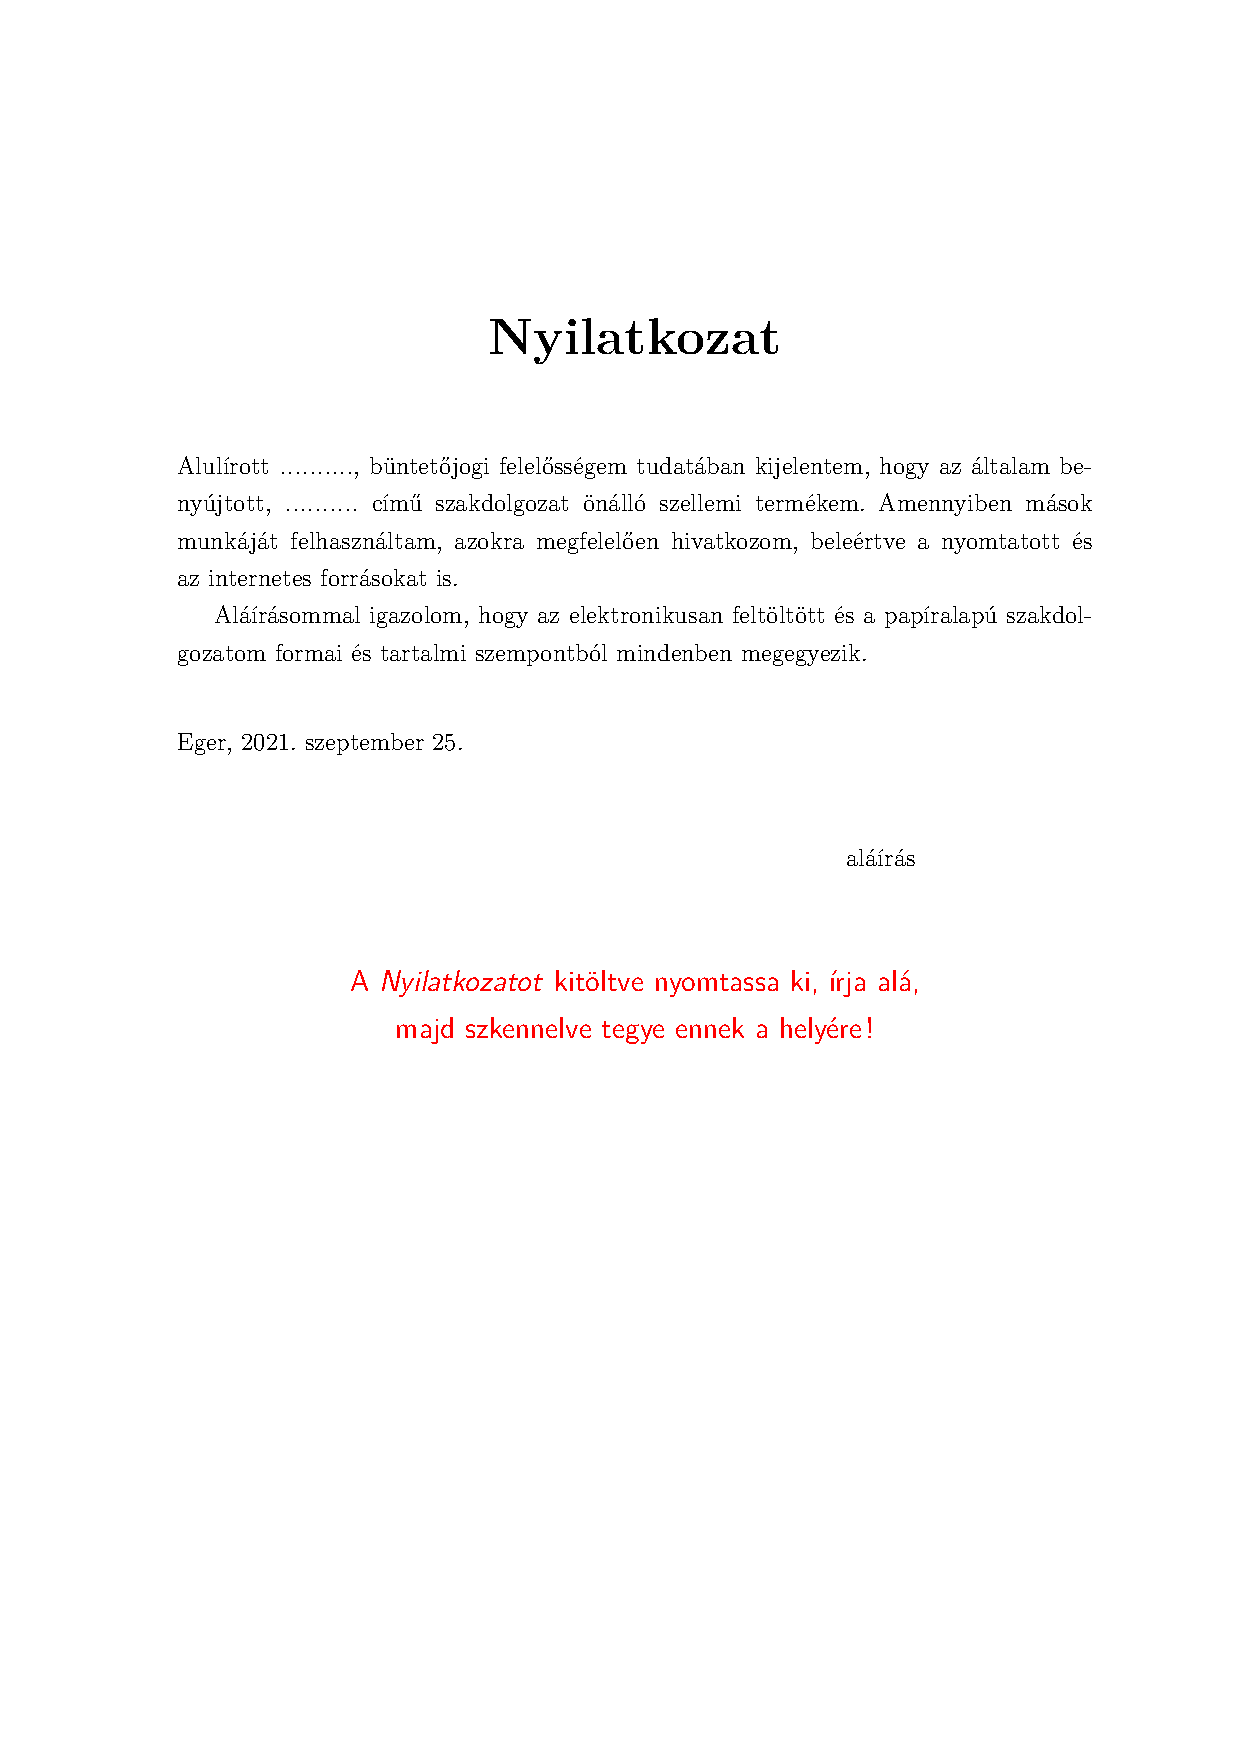
\includepdf{nyilatkozat.pdf}
\end{document}